\section{Casi d'uso}
In questa sezione vengono elencati i casi d'uso rilevati dall'analisi del capitolato \capitolato\ durante le riunioni con \RB\ e riguardanti l'\termine{SDK} e l'applicazione \termine{demo}. Questa consiste in una bolla lista della spesa condivisa, nella quale gli utenti sono divisi secondo le capacità di interazione con la lista.

Ogni caso d'uso è identificato dal seguente formalismo:
\begin{center}
	UC[\texttt{codice}]
\end{center}
dove \texttt{codice} è il codice gerarchico, numerico ed univoco, per identificare ogni caso d'uso.

\subsection{Attori}
Di seguito è riportato il diagramma \termine{UML} che descrive la gerarchia degli attori.

\subsubsection{Sviluppatore}
Viene definito \termine{sviluppatore} una qualsiasi persona che abbia accesso diretto all'\termine{SDK} e ai suoi contenuti, e che lo utilizzerà al fine di creare una applicazione che ne sfrutti le caratteristiche.

\subsubsection{Utente}
Viene definito utente una qualsiasi persona che utilizzi la bolla lista della spesa.
\subsubsection{Utente esterno}
Un utente esterno è una raffinazione del concetto di utente, e consiste in un utente che ha ricevuto una bolla lista della spesa tramite inoltro, e che quindi può solamente visualizzare la lista ma non interagirci in alcun modo.
\subsubsection{Utente senza permessi}
Un utente senza permessi è una raffinazione del concetto di utente, e consiste in un utente che ha ricevuto la bolla lista della spesa tramite pubblicazione, e che quindi può spuntare i prodotti di quest'ultima. Non può, però, modificare i prodotti presenti all'interno della lista.
\subsubsection{Utente con permessi}
Un utente con permessi è un utente che ha ricevuto la lista tramite pubblicazione. Può quindi spuntarne i prodotti e inoltre ha ricevuto, dal creatore della lista, l'autorizzazione a modificare,aggiungere o rimuovere prodotti dalla lista stessa.
\subsubsection{Creatore della lista}
Il creatore della lista gode di tutte le proprietà dell'utente con permessi, ma in aggiunta può decidere se mandare una bolla lista tramite inoltro o tramite pubblicazione e concedere permessi di modifica della lista agli utenti che ha invitato tramite pubblicazione, decidendo o meno la partecipazione attiva degli altri utenti.
\label{Attori}
\begin{figure}[ht]
	\centering
	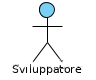
\includegraphics[scale=1]{Usecases/img/Attori.png}
	\caption{Attori dell'applicazione}
\end{figure}



\FloatBarrier
\subsection{Caso d'uso UC 0: \progetto (SDK)}
\label{Caso d'uso UC 0: \progetto (SDK)}
\begin{figure}[ht]
	\centering
	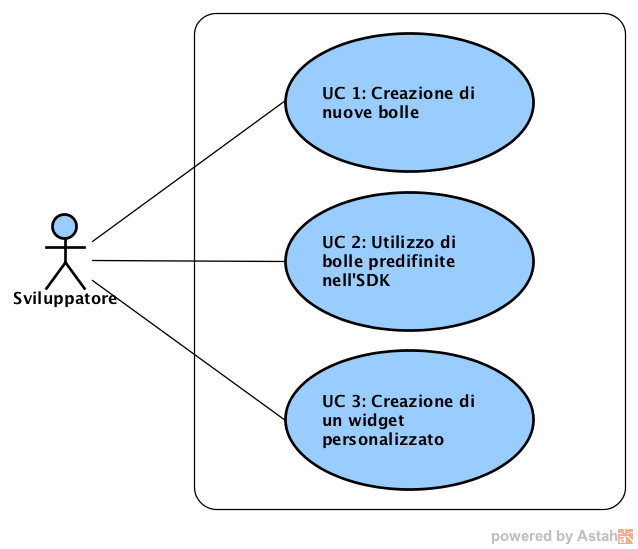
\includegraphics[scale=0.80]{Usecases/img/Monolith.png}
	\caption{Caso d'uso UC 0: \progetto(SDK)}
\end{figure}

\FloatBarrier
\begin{itemize}
\item \textbf{Attori:} Sviluppatore.
\item \textbf{Descrizione:} Tramite l'\termine{SDK} lo sviluppatore vuole:
	\begin{itemize}
	\item{Creare una nuova bolla utilizzando i widget dell'\termine{SDK}.}
	\item{Utilizzare una bolla predefinita.}
	\item{Creare un nuovo widget.}
	\end{itemize}
\item \textbf{Precondizione:} Lo sviluppatore ha accesso all'\termine{SDK}.
\item \textbf{Postcondizione:} Lo sviluppatore ha creato del codice eseguibile.
\item \textbf{Scenario Principale:}
	\begin{itemize}
	\item{Creazione di nuove bolle utilizzando i widget dell'\termine{SDK} (UC 1).}
	\item{Utilizzo di bolle predefinite nell'\termine{SDK} (UC 2).}
	\item{Creazione di un widget personalizzato (UC 3).}
	\end{itemize}
\end{itemize}
\newpage
\subsection{Caso d'uso UC 1: Creazione di nuove bolle}
\label{Caso d'uso UC 1: Creazione di nuove bolle}
\begin{figure}[ht]
	\centering
	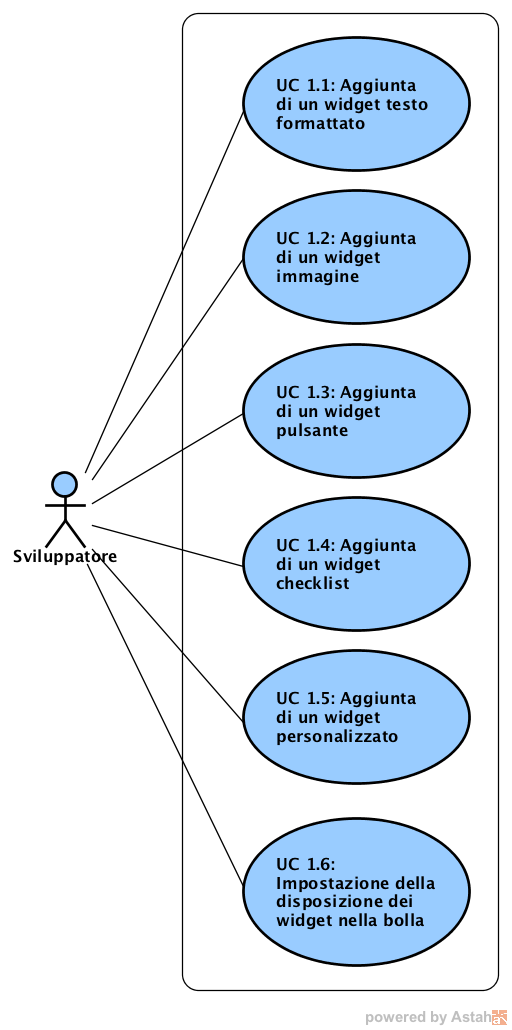
\includegraphics[scale=0.65]{Usecases/img/UC1.png}
	\caption{Caso d'uso UC 1: Creazione di nuove bolle}
\end{figure}

\FloatBarrier
\begin{itemize}
\item \textbf{Attori:} Sviluppatore;
\item \textbf{Descrizione:} Tramite l'\termine{SDK} lo sviluppatore vuole:
	\begin{itemize}
	\item{Aggiunta di un widget testo formattato a una bolla.} 
	\item{Aggiunta di un widget immagine a una bolla.}
	\item{Aggiunta di un widget bottone a una bolla.}
	\item{Aggiunta di un widget checklist a una bolla.}
	\item{Aggiunta di un widget personalizzato a una bolla.}
	\item{Impostare la disposizione dei widget nella bolla.}
	\end{itemize} 
\item \textbf{Precondizione:} Lo sviluppatore ha accesso all'\termine{SDK}.
\item \textbf{Postcondizione:} Lo sviluppatore ha creato del codice eseguibile. 
\item \textbf{Scenario principale:}
	\begin{itemize}
	\item{Lo sviluppatore vuole aggiungere a una bolla un widget testo formattato (UC 1.1).}
	\item{Lo sviluppatore vuole aggiungere a una bolla un widget immagine (UC 1.2).}
	\item{Lo sviluppatore vuole aggiungere a una bolla un widget pulsante (UC 1.3).}
	\item{Lo sviluppatore vuole aggiungere a una bolla un widget checklist (UC 1.4).}
	\item{Lo sviluppatore vuole aggiungere a una bolla un widget personalizzato (UC 1.5).}
	\item{Lo sviluppatore vuole impostare la disposizione dei wiget nella bolla (UC 1.6).}
	\end{itemize}
\end{itemize}
\subsubsection{Caso d'uso UC 1.1: Utilizzo di un widget testo formattato}
\label{Caso d'uso UC 1.1: Utilizzo di un widget testo formattato}

\begin{figure}[ht]
\centering
	\includegraphics[scale=0.6]{Usecases/img/{UC1.1}.png}
	\caption{Caso d'uso UC 1.1: Aggiunta di un widget testo formattato}
\end{figure}

\FloatBarrier
\begin{itemize}
\item\textbf{Attori}: Sviluppatore.
\item\textbf{Descrizione}: Lo sviluppatore vuole aggiungere a una bolla un widget testo formattato.
\item\textbf{Precondizione}: Lo sviluppatore ha accesso all'\termine{SDK}.
\item\textbf{Postcondizione}: Lo sviluppatore ha creato del codice eseguibile che permette di aggiungere a una bolla un widget testo formattato.
\item\textbf{Scenario principale}:
	\begin{itemize}
		\item Lo sviluppatore vuole scegliere la grandezza del font del testo (UC 1.1.1).
		\item Lo sviluppatore vuole impostare parte del testo in corsivo (UC 1.1.3).
		\item Lo sviluppatore vuole aggiungere un link cliccabile (UC 1.1.4).
		\item Lo sviluppatore vuole impostare parte del testo in grassetto (UC 1.1.7).
		\item Lo sviluppatore vuole impostare un colore a parte del testo (UC 1.1.8).
		\item Lo sviluppatore vuole aggiungere del testo alla bolla (1.1.10)
	\end{itemize}
	
\item\textbf{Scenario alternativo}
	\begin{itemize}
		\item Lo sviluppatore non inserisce la grandezza del font oppure la inserisce in modo non valido(UC 1.1.2).
		\item Lo sviluppatore non inserisce il colore del link cliccabile oppure lo inserisce in modo non valido(UC 1.1.6).
		\item Lo sviluppatore non imposta il colore del testo della bolla oppure lo inserisce in modo non valido(UC 1.1.9).
		\item Lo sviluppatore non inserisce del testo oppure lo inserisce in modo non valido(UC 1.1.11).
		
	\end{itemize}

\end{itemize}

\paragraph{Caso d'uso 1.1.1: Scelta della grandezza del font}
\begin{itemize}
\item\textbf{Attori}: Sviluppatore.
\item\textbf{Descrizione}: Lo sviluppatore vuole scegliere la grandezza del font della proprio widget.
\item\textbf{Precondizione}: Lo sviluppatore utilizza un widget testo formattato e vuole impostare la grandezza del font.
\item\textbf{Postcondizione}: Lo sviluppatore ha creato del codice eseguibile che permette di creare un widget testo formattato contenente del testo con la grandezza del font impostata.
\item\textbf{Estensioni:}
	\begin{itemize}
		\item Impostazione della grandezza del font a default (UC 1.1.2).
	\end{itemize}
\item\textbf{Scenario principale}: Lo sviluppatore utilizza un widget testo formattato e vuole impostare la grandezza del font. 
\item\textbf{Scenari alternativi}: La grandezza del font viene impostata a default (UC 1.1.2).
\end{itemize}
\paragraph{Caso d'uso 1.1.2: Impostazione della grandezza del font a default}
\begin{itemize}
\item\textbf{Attori}: Sviluppatore.
\item\textbf{Descrizione}: Se lo sviluppatore non ha impostato la grandezza del font o lo ha impostato con una grandezza non valida il font viene configurato ad un valore di default.
\item\textbf{Precondizione}: Lo sviluppatore ha impostato una grandezza del font non valida alla bolla di tipo testo formattato o non ha impostato alcuna grandezza al font.
\item\textbf{Postcondizione}: Lo sviluppatore ha creato del codice eseguibile cSe lo sviluppatore non ha impostato il colore del link o lo ha impostato con una colore non valido il link viene impostato con il colore blu.he permette di creare una bolla di testo formattato contenente del testo con una grandezza del font impostata a default.
\end{itemize}
\paragraph{Caso d'uso 1.1.3: Visualizzazione di parte del testo in corsivo}
\begin{itemize}
\item\textbf{Attori}: Sviluppatore.
\item\textbf{Descrizione}: Lo sviluppatore vuole impostare in corsivo parte del testo di una bolla di tipo testo formattato.
\item\textbf{Precondizione}: Lo sviluppatore utilizza una bolla di testo formattato e vuole impostare parte del testo in corsivo.
\item\textbf{Postcondizione}: Lo sviluppatore ha creato codice eseguibile per creare una bolla di tipo testo formattato che contiene parte del testo in corsivo.
\end{itemize}
\paragraph{Caso d'uso 1.1.4: Aggiunta di link cliccabili}
\begin{itemize}
\item\textbf{Attori}: Sviluppatore.
\item\textbf{Descrizione}: Lo sviluppatore vuole aggiungere un link cliccabile ad una bolla di tipo testo formattato che porti l'utente a visualizzare una pagina web esterna alla bolla stessa.
\item\textbf{Precondizione}: Lo sviluppatore utilizza una bolla di testo formattato e vuole aggiungere un link cliccabile.
\item\textbf{Postcondizione}: Lo sviluppatore ha creato codice eseguibile che permette di creare una bolla di testo formattato che contiene un link cliccabile.

\item\textbf{Inclusioni:}
	\begin{itemize}
		\item Lo sviluppatore seleziona il colore del link cliccabile (UC 1.1.5).
	\end{itemize}

	
\end{itemize}
\paragraph{Caso d'uso 1.1.5: Impostazione del colore del link}
\begin{itemize}
\item\textbf{Attori}: Sviluppatore.
\item\textbf{Descrizione}: Lo sviluppatore vuole selezionare il colore di un link cliccabile prima che esso venga cliccato da parte dell'utente finale della bolla.
\item\textbf{Precondizione}: Lo sviluppatore utilizza una bolla di tipo testo formattato con presente al suo interno un link cliccabile di cui vuole impostare il colore.
\item\textbf{Postcondizione}: Lo sviluppatore ha creato codice eseguibile che permette di creare una bolla di testo formattato contenente un link cliccabile che viene visualizzato con il colore impostato.

\item\textbf{Estensioni:}
	\begin{itemize}
		\item Impostazione del colore del link a blu (UC 1.1.6).
	\end{itemize}
\end{itemize}
\paragraph{Caso d'uso 1.1.6: Impostazione del colore del link a blu}
\begin{itemize}
\item\textbf{Attori}: Sviluppatore.
\item\textbf{Descrizione}: Se lo sviluppatore non ha impostato il colore del link o lo ha impostato con una colore non valido il link viene impostato con il colore blu.
\item\textbf{Precondizione}: Lo sviluppatore ha impostato un colore non valido al link di una bolla di tipo testo formattato o non ha impostato alcun colore al link.
\item\textbf{Postcondizione}: Il testo del link cliccabile viene impostato a blu.
\end{itemize}
\paragraph{Caso d'uso 1.1.7: Visualizzazione di parte del testo in grassetto}
\begin{itemize}
\item\textbf{Attori}: Sviluppatore.
\item\textbf{Descrizione}: Lo sviluppatore vuole impostare in grassetto parte del testo di un widget testo formattato.
\item\textbf{Precondizione}: Lo sviluppatore utilizza un widget testo formattato e vuole impostare parte del testo in grassetto.
\item\textbf{Postcondizione}: Lo sviluppatore ha creato codice eseguibile che permette di creare un widget testo formattato contenente parte del testo in grassetto.
\item\textbf{Scenario principale}: Lo sviluppatore vuole impostare in grassetto parte del testo di un widget testo formattato.
\end{itemize}
\paragraph{Caso d'uso 1.1.8: Impostazione del colore di parte del testo}
\begin{itemize}
\item\textbf{Attori}: Sviluppatore.
\item\textbf{Descrizione}: Lo sviluppatore vuole impostare un colore a parte del testo di una bolla di testo formattato.
\item\textbf{Precondizione}: Lo sviluppatore utilizza una bolla di tipo testo formattato e vuole impostare un colore colore personalizzato al testo.
\item\textbf{Postcondizione}: Lo sviluppatore ha creato codice eseguibile che permette di creare una bolla di testo formattato contenente una parte del testo visualizzato con il colore impostato.
\item\textbf{Estensioni:}
	\begin{itemize}
		\item Visualizzazione di un messaggio d'errore (UC 1.1.9).
		\end{itemize}

\end{itemize}
\paragraph{Caso d'uso 1.1.9 Impostazione del colore del testo a default}
\begin{itemize}
\item\textbf{Attori}: Sviluppatore.
\item\textbf{Descrizione}: Se lo sviluppatore non imposta il colore del font o lo imposta con un colore non valido il colore del font viene configurato ad un valore di default.
\item\textbf{Precondizione}: Lo sviluppatore vuole impostare un colore al testo di un widget tipo testo formattato non valido o non ha impostato alcun colore al testo.
\item\textbf{Postcondizione}: Il colore del testo viene impostato ad un valore di default.
\item\textbf{Scenario principale}: Lo sviluppatore ha commesso un errore nell'impostazione del colore del testo, perciò questo viene impostato a default.
\end{itemize}
\paragraph{Caso d'uso 1.1.10: Aggiunta di testo al widget}
\begin{itemize}
\item\textbf{Attori}: Sviluppatore.
\item\textbf{Descrizione}: Lo sviluppatore vuole aggiungere del testo a un widget testo formattato già esistente.
\item\textbf{Precondizione}: Lo sviluppatore vuole utilizzare un widget testo formattato e vuole aggiungere del testo a tale widget.
\item\textbf{Postcondizione}: Lo sviluppatore ha creato codice eseguibile che permette di aggiungere del testo ad un widget testo formattato già esistente.
\item\textbf{Estensioni:}
	\begin{itemize}
		\item Visualizzazione di un messaggio d'errore (UC 1.1.11).
		\end{itemize}
\item\textbf{Scenario principale}: Lo sviluppatore vuole aggiungere del testo a un widget testo formattato già esistente.
\item\textbf{Scenari alternativi}: 
	\begin{itemize}
	\item Viene visualizzato un messaggio d'errore (UC 1.1.11).
	\end{itemize}
\end{itemize}
\paragraph{Caso d'uso 1.1.11 Visualizzazione messaggio d'errore}
\begin{itemize}
\item\textbf{Attori}: Sviluppatore.
\item\textbf{Descrizione}: Lo sviluppatore viene avvisato con un messaggio d'errore dell'aggiunta in modo errato di ulteriore testo nel widget testo formattato.
\item\textbf{Precondizione}: Lo sviluppatore ha aggiunto in modo errato del testo in un widget testo formattato.
\item\textbf{Postcondizione}: Viene visualizzato un messaggio d'errore.
\item\textbf{Scenario principale}: Lo sviluppatore visualizza un messaggio d'errore.
\end{itemize}

\subsubsection{Caso d'uso UC 1.2: Utilizzo di una bolla di tipo bottone}
\label{Caso d'uso UC 1.2: Utilizzo di una bolla di tipo bottone}
\begin{figure}[ht]
	\centering
	\includegraphics[scale=0.80]{Usecases/img/{UC1.2}.png}
	\caption{Caso d'uso UC 1.2: Utilizzo di una bolla di tipo bottone}
\end{figure}
\FloatBarrier
\begin{itemize}
\item\textbf{Attori}: Sviluppatore.
\item\textbf{Descrizione}: Lo sviluppatore vuole utilizzare una bolla di tipo bottone.
\item\textbf{Precondizione}: Lo sviluppatore vuole utilizzare una bolla di tipo bottone.
\item\textbf{Postcondizione}: Lo sviluppatore crea codice eseguibile per creare una bolla di tipo bottone.
\item\textbf{Scenario principale}:
	\begin{itemize}
		\item Lo sviluppatore vuole utilizzare una bolla di tipo \termine{bottone semplice}(UC 1.2.1).
		\item Lo sviluppatore vuole utilizzare una bolla di tipo \termine{checkbutton}(UC 1.2.2).
		\item Lo sviluppatore vuole impostare una reazione ad un evento del bottone(UC 1.2.3).
	\end{itemize}

\end{itemize}


\paragraph{Caso d'uso UC 1.2.1: Utilizzo di una bolla di tipo bottone semplice}
\label{UC 1.2.1: Utilizzo di una bolla di tipo bottone semplice}
\begin{figure}[ht]
	\centering
	\includegraphics[scale=0.54]{Usecases/img/{UC1.2.1}.png}
	\caption{Caso d'uso UC 1.2.1: Utilizzo di una bolla di tipo bottone semplice}
\end{figure}
\FloatBarrier
\begin{itemize}
\item\textbf{Attori}: Sviluppatore.
\item\textbf{Descrizione}: Lo sviluppatore vuole utilizzare una bolla di tipo bottone semplice.
\item\textbf{Precondizione}: Lo sviluppatore vuole utilizzare una bolla di tipo bottone semplice.
\item\textbf{Postcondizione}: Lo sviluppatore ha generato del codice eseguibile per creare una bolla di tipo bottone semplice con i parametri scelti.

\item\textbf{Scenario principale}:
	\begin{itemize}
		\item Lo sviluppatore vuole impostare il testo del bottone (UC 1.2.1.1).
		\item Lo sviluppatore vuole impostare le dimensioni del bottone (UC1.2.1.3).
		\item Lo sviluppatore vuole impostare il colore di sfondo del bottone(UC1.2.1.5).
	\end{itemize}
\end{itemize}

\paragraph{Caso d'uso UC 1.2.3: Visualizzazione messaggio d'errore}

\FloatBarrier
\begin{itemize}
\item\textbf{Attori}: Sviluppatore.
\item\textbf{Descrizione}: Lo sviluppatore visualizza un messaggio d'errore.
\item\textbf{Precondizione}: Lo sviluppatore ha inserito in modo errato un immagine o non ha definito l'immagine da aggiungere.
\item\textbf{Postcondizione}: Viene visualizzato un messaggio d'errore.
\item\textbf{Scenario principale}: Lo sviluppatore ha inserito in modo non valido un immagine o non ha definito l'immagine da aggiungere, perciò viene visualizzato un errore.
\end{itemize}

\newpage
\paragraph{Caso d'uso UC 1.2.3: Impostazione della reazione ad un evento del bottone}
\label{UC 1.2.3: Impostazione della reazione ad un evento del bottone}
\begin{figure}[ht]
	\centering
	\includegraphics[scale=0.54]{Usecases/img/{UC1.2.3}.png}
	\caption{Caso d'uso UC 1.2.3: Impostazione della reazione ad un evento del bottone}
\end{figure}
\FloatBarrier
\begin{itemize}
\item\textbf{Attori}: Sviluppatore.
\item\textbf{Descrizione}: Lo sviluppatore vuole collegare una reazione ad un qualsiasi evento associato al bottone.
\item\textbf{Precondizione}: Lo sviluppatore utilizza un bottone e vuole associarci un evento.
\item\textbf{Postcondizione}: Lo sviluppatore ha associato un evento al bottone oppure non l'ha associato.
\item\textbf{Scenario principale}:
	\begin{itemize}
		\item Lo sviluppatore vuole collegare una reazione all'evento "click normale" del bottone (ossia un semplice click sul bottone) (UC 1.2.3.1).
		\item Lo sviluppatore vuole collegare una reazione all'evento "click prolungato" del bottone (ossia un click che ha una certa rilevanza di tempo sul bottone) (UC1.2.3.2).
	\end{itemize}
\end{itemize}

\paragraph{Caso d'uso UC 1.2.4: Impostazione di altezza e larghezza dell'immagine a default}

\FloatBarrier
\begin{itemize}
\item\textbf{Attori}: Sviluppatore.
\item\textbf{Descrizione}: Lo sviluppatore ha impostato in modo non valido le dimensioni di altezza e/o lunghezza dell'immagine vengono impostate le dimensioni ai valori di default.
\item\textbf{Precondizione}: Lo sviluppatore ha impostato in modo non valido la dimensione di altezza e/o lunghezza dell'immagine.
\item\textbf{Postcondizione}: Vengono impostate le dimensioni di altezza e larghezza dell'immagine ai valori di default.
\item\textbf{Scenario principale}: Lo sviluppatore ha impostato in modo non valido la dimensione di altezza e/o lunghezza dell'immagine, perciò queste vengono impostate a default.
\end{itemize}




\newpage
\subsubsection{Caso d'uso UC 1.3: Aggiunta di un widget bottone}
\label{Caso d'uso UC 1.3: Aggiunta di un widget bottone}
\begin{figure}[ht]
	\centering
	\includegraphics[scale=0.6]{Usecases/img/{UC1.3}.png}
	\caption{Caso d'uso UC 1.3: Aggiunta di un widget bottone}
\end{figure}
\FloatBarrier
\begin{itemize}
\item\textbf{Attori}: Sviluppatore.
\item\textbf{Descrizione}: Lo sviluppatore vuole aggiungere un widget bottone a una bolla per creare del codice eseguibile.
\item\textbf{Precondizione}: Lo sviluppatore vuole aggiungere un widget bottone a una bolla.
\item\textbf{Postcondizione}: Lo sviluppatore crea codice eseguibile per creare una bolla di tipo bottone.
\item\textbf{Scenario principale}:
	\begin{itemize}
		\item Lo sviluppatore vuole aggiungere un widget \termine{bottone semplice}(UC 1.3.1).
		\item Lo sviluppatore vuole aggiungere un widget \termine{checkbutton}(UC 1.3.2).
		\item Lo sviluppatore vuole impostare una reazione ad un evento del bottone(UC 1.3.3).
	\end{itemize}

\end{itemize}
\newpage
\paragraph{Caso d'uso UC 1.3.1: Aggiunta di un widget bottone semplice}
\label{UC 1.3.1: Aggiunta di un widget bottone semplice}
\begin{figure}[ht]
	\centering
	\includegraphics[scale=0.54]{Usecases/img/{UC1.3.1}.png}
	\caption{Caso d'uso UC 1.3.1: Aggiunta di un widget bottone semplice}
\end{figure}
\FloatBarrier
\begin{itemize}
\item\textbf{Attori}: Sviluppatore.
\item\textbf{Descrizione}: Lo sviluppatore vuole utilizzare un widget bottone semplice.
\item\textbf{Precondizione}: Lo sviluppatore vuole utilizzare un widget bottone semplice.
\item\textbf{Postcondizione}: Lo sviluppatore ha generato del codice eseguibile per creare un widget bottone semplice con i parametri scelti.

\item\textbf{Scenario principale}:
	\begin{itemize}
		\item Lo sviluppatore vuole impostare il testo del bottone (UC 1.3.1.1).
		\item Lo sviluppatore vuole impostare le dimensioni del bottone (UC1.3.1.3).
		\item Lo sviluppatore vuole impostare il colore di sfondo del bottone(UC1.3.1.5).
	\end{itemize}
	
\item\textbf{Scenari alternativi}:	
	\begin{itemize}
		\item Lo sviluppatore non inserisce del testo nelwidget o lo inserisce in modo non valido(UC 1.3.1.3).
		\item Lo sviluppatore non inserisce le dimensioni del bottone oppure le inserisce in modo non valido(UC 1.3.1.4).
		\item Lo sviluppatore non inserisce un colore di sfondo del bottone oppure lo inserisce in modo non valido(UC 1.3.1.6).
	\end{itemize}
	
\end{itemize}

\subparagraph{Caso d'uso UC 1.3.1.1: Visualizzazione come elenco numerato}

\FloatBarrier
\begin{itemize}
\item\textbf{Attori}: Sviluppatore.
\item\textbf{Descrizione}: Lo sviluppatore vuole impostare lo stile di visualizzazione della lista mediante dei numeri ordinati in modo crescente.
\item\textbf{Precondizione}: Lo sviluppatore vuole impostare lo stile di visualizzazione della lista come elenco numerato.
\item\textbf{Postcondizione}: Lo sviluppatore ha impostato lo stile di visualizzazione della lista come elenco numerato.
\end{itemize}

\subparagraph{Caso d'uso UC 1.3.1.2: Visualizzazione come elenco non numerato con indicatore "pallino"}

\FloatBarrier
\begin{itemize}
\item\textbf{Attori}: Sviluppatore.
\item\textbf{Descrizione}: Lo sviluppatore vuole impostare lo stile di visualizzazione di una lista come un elenco non numerato usando come indicatore "pallino".
\item\textbf{Precondizione}: Lo sviluppatore vuole impostare lo stile di visualizzazione di una lista come elenco puntato.
\item\textbf{Postcondizione}: Lo sviluppatore ha impostato lo stile di visualizzazione della lista come elenco puntato usando come indicatore "pallino".
\end{itemize}

\subparagraph{Caso d'uso UC 1.3.1.3: Impostazione delle dimensioni del bottone}

\FloatBarrier
\begin{itemize}
\item\textbf{Attori}: Sviluppatore.
\item\textbf{Descrizione}: Lo sviluppatore vuole impostare le dimensioni del bottone.
\item\textbf{Precondizione}: Lo sviluppatore utilizza un widget bottone semplice e vuole impostare le dimensioni del bottone.
\item\textbf{Postcondizione}: Lo sviluppatore crea del codice eseguibile per creare un widget bottone semplice contenente un bottone dalle dimensioni specificate.
\item \textbf{Estensioni}: 
\begin{itemize}
\item Impostazione delle dimensioni del bottone a default (UC 1.3.1.4).
\end{itemize}
\item \textbf{Scenario principale}: Lo sviluppatore imposta le dimensioni del bottone.
\item \textbf{Scenari alternativi}: Le dimensioni del bottone vengono impostate a default (UC 1.3.1.4).
\end{itemize}
\subparagraph{Caso d'uso UC 1.3.1.4: Impostazione delle dimensioni del bottone a default}

\FloatBarrier
\begin{itemize}
\item\textbf{Attori}: Sviluppatore.
\item\textbf{Descrizione}: Se lo sviluppatore imposta delle dimensioni del bottone non valide o non imposta alcuna dimensione la dimensione del bottone viene impostata ad un valore di default.
\item\textbf{Precondizione}: Lo sviluppatore non ha impostato delle dimensioni per il bottone o ha inserito delle dimensioni non valide.
\item\textbf{Postcondizione}: Le dimensioni del bottone vengono impostate ad un valore di default.
\item\textbf{Scenario principale}: Lo sviluppatore non ha impostato delle dimensioni per il bottone o ha inserito delle dimensioni non valide, perciò le dimensioni del bottone vengono impostate ad un valore di default.
\end{itemize}


\subparagraph{Caso d'uso UC 1.3.1.5: Impostazione del colore di sfondo del bottone}

\FloatBarrier
\begin{itemize}
\item\textbf{Attori}: Sviluppatore.
\item\textbf{Descrizione}: Lo sviluppatore vuole impostare il colore di sfondo del bottone.
\item\textbf{Precondizione}: Lo sviluppatore vuole utilizzare un widget bottone semplice e vuole impostare un colore personalizzato al bottone in essa contenuto.
\item\textbf{Postcondizione}: Lo sviluppatore ha creato del codice eseguibile per creare un widget bottone semplice contenente un bottone con il colore di sfondo impostato.
\item\textbf{Estensioni}: 
\begin{itemize}
\item Impostazione del colore del bottone a default (UC 1.3.1.6).
\end{itemize}
\item\textbf{Scenario principale}: Lo sviluppatore imposta il colore di sfondo del bottone.
\item\textbf{Scenari alternativi}: Il colore di sfondo del bottone viene impostato a default (UC 1.3.1.6).
\end{itemize}

\subparagraph{Caso d'uso UC 1.3.1.6: Impostazione del colore del bottone a default}

\FloatBarrier
\begin{itemize}
\item\textbf{Attori}: Sviluppatore.
\item\textbf{Descrizione}: Se lo sviluppatore ha impostato un colore di sfondo non valido per il bottone o non è stato impostato alcun colore allora il bottone viene impostato con il colore di default.
\item\textbf{Precondizione}: Lo sviluppatore ha impostato un colore di sfondo non valido al bottone o non è stato specificato alcun colore.
\item\textbf{Postcondizione}: Il colore di sfondo del bottone di un widget bottone semplice viene impostato con il colore di default.
\item\textbf{Scenario principale}: Lo sviluppatore ha impostato un colore di sfondo non valido al bottone o non è stato specificato alcun colore, perciò il colore di sfondo del bottone viene impostato con il colore di default.
\end{itemize}

\newpage
\paragraph{Caso d'uso UC 1.3.2: Aggiunta di un widget checkbutton}
\label{UC 1.3.2: Aggiunta di un widget checkbutton}
\begin{figure}[ht]
	\centering
	\includegraphics[scale=0.70]{Usecases/img/{UC1.3.2}.png}
	\caption{Caso d'uso UC 1.3.2: Aggiunta di un widget checkbutton}
\end{figure}
\FloatBarrier
\begin{itemize}
\item\textbf{Attori}: Sviluppatore.
\item\textbf{Descrizione}: Lo sviluppatore vuole utilizzare un bottone particolare che possiede due stati: "clicked" e "unclicked".
\item\textbf{Precondizione}: Lo sviluppatore vuole utilizzare un widget checkbutton.
\item\textbf{Postcondizione}: Lo sviluppatore he generato codice eseguibile per creare un widget checkbutton con i parametri scelti.
\item\textbf{Scenario principale}:
	\begin{itemize}
		\item Lo sviluppatore vuole impostare lo stato del bottone (UC 1.3.2.1).
		\item Lo sviluppatore non imposta lo stato del bottone (UC 1.3.2.2).
		\item Lo sviluppatore vuole personalizzare il bottone (UC 1.3.2.3).
	\end{itemize}
\end{itemize}

\subparagraph{Caso d'uso UC 1.3.2.1: Impostazione dello stato del checklistitem}
\label{UC 1.3.2.1: Impostare lo stato del bottone}
\FloatBarrier
\begin{itemize}
\item\textbf{Attori}: Sviluppatore.
\item\textbf{Descrizione}: Lo sviluppatore vuole modificare lo stato del bottone. Questo può essere di 2 tipi: "cliccato" e "non cliccato".
\item\textbf{Precondizione}: Lo sviluppatore utilizza un widget checklistitem e vuole cambiarne lo stato del bottone.
\item\textbf{Postcondizione}: Lo sviluppatore ha cambiato lo stato del bottone di un widget checklistitem.
\item\textbf{Estensioni}: 
\begin{itemize}
\item Impostazione automatica del bottone nello stato "non cliccato" (UC 1.3.2.2).
\end{itemize}
\item\textbf{Scenario principale}: Lo sviluppatore imposta lo stato del bottone.
\item\textbf{Scenari alternativi}: Lo stato del bottone viene impostato automaticamente su "non cliccato" (UC 1.3.2.2).
\end{itemize}

\subparagraph{Caso d'uso UC 1.3.2.2: Impostazione del bottone nello stato "non cliccato"}
\label{UC 1.3.2.2: Impostazione del bottone nello stato "non cliccato"}

\FloatBarrier
\begin{itemize}
\item\textbf{Attori}: Sviluppatore.
\item\textbf{Descrizione}: Se lo sviluppatore non ha impostato lo stato del bottone viene impostato a "non cliccato".
\item\textbf{Precondizione}: Lo sviluppatore utilizza un widget checkbutton e non ha impostato lo stato del bottone.
\item\textbf{Postcondizione}: Lo stato del bottone viene impostato a "non cliccato".
\item\textbf{Scenario principale}: Lo sviluppatore non ha impostato lo stato del bottone, perciò questo viene impostato a "non cliccato".
\end{itemize}

\subparagraph{Caso d'uso UC 1.3.2.3: Personalizzazione del bottone}
\label{UC 1.3.2.3: Personalizzazione del bottone}
\begin{figure}[ht]
	\centering
	\includegraphics[scale=0.50]{Usecases/img/{UC1.3.2.3}.png}
	\caption{Caso d'uso UC 1.3.2.3: Personalizzazione del bottone}
\end{figure}
\FloatBarrier
\begin{itemize}
\item\textbf{Attori}: Sviluppatore.
\item\textbf{Descrizione}: Lo sviluppatore vuole personalizzare la modalità in cui il bottone viene visualizzato.
\item\textbf{Precondizione}: Lo sviluppatore utilizza un widget checklistitem.
\item\textbf{Postcondizione}: Lo sviluppatore ha personalizzato la modalità di visualizzazione del checklistitem.
\item\textbf{Scenario principale}:
	\begin{itemize}
		\item Visualizzazione del flag mediante una "x" (UC 1.3.2.3.1).
		\item Visualizzazione del flag mediante una spunta (UC1.3.2.3.2).
		\item Visualizzazione del flag mediante una colorazione del bottone (UC1.3.2.3.3).
	\end{itemize}
	\item\textbf{Scenario alternativo}:
	\begin{itemize}
		\item Lo sviluppatore non imposta il colore del flag oppure lo imposta in modo non valido (UC 1.3.2.3.5).
	\end{itemize}
\end{itemize}

\subsubparagraph{Caso d'uso UC 1.3.2.3.1: Visualizzazione del flag mediante una "v"}

\FloatBarrier
\begin{itemize}
\item\textbf{Attori}: Sviluppatore.
\item\textbf{Descrizione}: Lo sviluppatore vuole impostare la visualizzazione del flag mediante una "v".
\item\textbf{Precondizione}: Lo sviluppatore utilizza un widget checkbutton e vuole impostarne la visualizzazione del flag mediante una "v".
\item\textbf{Postcondizione}: Lo sviluppatore ha impostato la visualizzazione del flag mediante una "v".
\item\textbf{Scenario principale}: Lo sviluppatore vuole impostare la visualizzazione del flag mediante una "v".
\end{itemize}

\subsubparagraph{Caso d'uso UC 1.3.2.3.2: Visualizzazione del flag mediante una "x"}

\FloatBarrier
\begin{itemize}
\item\textbf{Attori}: Sviluppatore.
\item\textbf{Descrizione}: Lo sviluppatore vuole impostare la visualizzazione del flag mediante una "x".
\item\textbf{Precondizione}: Lo sviluppatore utilizza un widget checkbutton e vuole impostarne la visualizzazione del flag mediante una "x".
\item\textbf{Postcondizione}: Lo sviluppatore ha impostato la visualizzazione del flag mediante una "x".
\item\textbf{Scenario principale}: Lo sviluppatore vuole impostare la visualizzazione del flag mediante una "x".
\end{itemize}

\subparagraph{Caso d'uso UC 1.3.2.3.3: Impostazione del colore di sfondo del box di spunta a bianco}

\FloatBarrier
\begin{itemize}
\item\textbf{Attori}: Sviluppatore.
\item\textbf{Descrizione}: Lo sviluppatore ha inserito il carattere di spunta e il colore di sfondo del box di spunta viene impostato automaticamente a bianco.
\item\textbf{Precondizione}: Lo sviluppatore ha impostato il carattere di spunta.
\item\textbf{Postcondizione}: Lo sviluppatore ha impostato il carattere di spunta e il colore di sfondo del box di spunta è stato impostato automaticamente a bianco.
\item\textbf{Scenario principale}: Lo sviluppatore ha inserito il carattere di spunta e il colore di sfondo del box di spunta viene impostato automaticamente a bianco.
\end{itemize}
\subsubparagraph{Caso d'uso UC 1.3.2.3.4: Scelta del colore di "check"}

\FloatBarrier
\begin{itemize}
\item\textbf{Attori}: Sviluppatore;
\item\textbf{Descrizione}: Lo sviluppatore vuole impostare la colorazione del check del bottone.
\item\textbf{Precondizione}: Lo sviluppatore utilizza un widget checkbutton di cui vuole impostarne la colorazione mediante cui visualizzare il "check".
\item\textbf{Postcondizione}: Lo sviluppatore ha impostato il colore della colorazione del bottone mediante cui visualizzare il "check".
\item \textbf{Estensioni}: 
\begin{itemize}
\item Impostazione del colore di check a verde (UC 1.3.2.3.5).
\end{itemize}
\item\textbf{Scenario principale}: Lo sviluppatore imposta il colore mediante il quale visualizza il "check".
\item\textbf{Scenari alternativi}: Il colore di "check" viene impostato a verde (UC 1.3.2.3.5).
\end{itemize}
\subsubparagraph{Caso d'uso UC 1.3.2.3.5: Impostazione del colore del flag a verde}

\FloatBarrier
\begin{itemize}
\item\textbf{Attori}: Sviluppatore.
\item\textbf{Descrizione}: Lo sviluppatore non seleziona alcuna colorazione del checkbutton mediante cui visualizzare il flag ed allora questa viene impostata a verde.
\item\textbf{Precondizione}: Lo sviluppatore non ha scelto il colore del checkbutton mediante cui visualizzare il flag.
\item\textbf{Postcondizione}: Il colore del checkbutton mediante cui visualizzare il flag viene impostato a verde.
\item\textbf{Scenario principale}: Lo sviluppatore commette un errore nella selezione del colore di del flag, perciò questo viene impostato a verde. 
\end{itemize}

\newpage
\paragraph{Caso d'uso UC 1.3.3: Impostazione della reazione ad un evento del bottone}
\label{UC 1.3.3: Impostazione della reazione ad un evento del bottone}
\begin{figure}[ht]
	\centering
	\includegraphics[scale=0.54]{Usecases/img/{UC1.3.3}.png}
	\caption{Caso d'uso UC 1.3.3: Impostazione della reazione ad un evento del bottone}
\end{figure}
\FloatBarrier
\begin{itemize}
\item\textbf{Attori}: Sviluppatore.
\item\textbf{Descrizione}: Lo sviluppatore vuole collegare una reazione ad un qualsiasi evento associato al bottone.
\item\textbf{Precondizione}: Lo sviluppatore utilizza un bottone e vuole associarci un evento.
\item\textbf{Postcondizione}: Lo sviluppatore ha associato un evento al bottone.
\item\textbf{Scenario principale}:
	\begin{itemize}
		\item Lo sviluppatore vuole collegare una reazione all'evento "click normale" del bottone (ossia un semplice click sul bottone) (UC 1.3.3.1).
		\item Lo sviluppatore vuole collegare una reazione all'evento "click prolungato" del bottone (ossia un click che ha una certa rilevanza di tempo sul bottone) (UC1.3.3.2).
	\end{itemize}
	\item\textbf{Scenario alternativo}:
	\begin{itemize}
		\item Lo sviluppatore non imposta un timer all'evento "click prolungato" oppure lo imposta in modo non corretto (UC 1.3.3.4).
	\end{itemize}
\end{itemize}

\subparagraph{Caso d'uso UC 1.3.3.1: Collegamento di una reazione all'evento "click normale" del bottone}

\FloatBarrier
\begin{itemize}
\item\textbf{Attori}: Sviluppatore.
\item\textbf{Descrizione}: Lo sviluppatore vuole collegare un reazione all'evento "click normale" del bottone. Per "click normale" si intende un normale click sul bottone stesso.
\item\textbf{Precondizione}: Lo sviluppatore utilizza un bottone.
\item\textbf{Postcondizione}: Lo sviluppatore ha associato una reazione all'evento "click normale" del bottone.
\item\textbf{Scenario principale}: Lo sviluppatore associa una reazione all'evento "click normale" del bottone.
\end{itemize}

\subparagraph{Caso d'uso UC 1.3.3.2: Collegamento di una reazione all'evento "click prolungato" del bottone}

\FloatBarrier
\begin{itemize}
\item\textbf{Attori}: Sviluppatore.
\item\textbf{Descrizione}: Lo sviluppatore vuole collegare un reazione all'evento "click prolungato" del bottone. Per "click prolungato" si intende un click che ha una certa rilevanza di tempo sul bottone stesso.
\item\textbf{Precondizione}: Lo sviluppatore utilizza un bottone.
\item\textbf{Postcondizione}: Lo sviluppatore ha associato una reazione all'evento di "click prolungato" del bottone.
\item \textbf{Inclusioni}:
\begin{itemize}
\item Impostazione del timer per l'attivazione dell'evento (UC 1.3.3.3).
\end{itemize} 
\item\textbf{Scenario principale}: Lo sviluppatore associa una reazione all'evento "click prolungato" del bottone.
\end{itemize}

\subparagraph{Caso d'uso UC 1.3.3.3: Impostazione del timer per l'attivazione dell'evento}

\FloatBarrier
\begin{itemize}
\item\textbf{Attori}: Sviluppatore.
\item\textbf{Descrizione}: Lo sviluppatore vuole impostare un timer per l'attivazione dell'evento associato al click prolungato.
\item\textbf{Precondizione}: Lo sviluppatore vuole impostare un evento al click prolungato del bottone.
\item\textbf{Postcondizione}: Lo sviluppatore ha impostato un timer per l'attivazione dell'evento associato al click prolungato del bottone.
\item \textbf{Estensioni}: 
\begin{itemize}
\item Impostazione del valore del timer a default (UC 1.3.3.4).
\end{itemize}
\item\textbf{Scenario principale}: Lo sviluppatore imposta un timer per l'attivazione dell'evento associato al click prolungato.
\item\textbf{Scenari alternativi}: Il timer viene impostato a default (UC 1.3.3.4).
\end{itemize}

\subparagraph{Caso d'uso UC 1.3.3.4: Impostazione del valore del timer a default}

\FloatBarrier
\begin{itemize}
\item\textbf{Attori}: Sviluppatore.
\item\textbf{Descrizione}: Se lo sviluppatore non ha impostato il valore del timer dell'evento il relazione al click prolungato sul bottone allora il valore del timer viene impostato a default. Per default si intende impostato a 0 (unità di misura ancora da decidere). 
\item\textbf{Precondizione}: Lo sviluppatore non ha impostato il timer dell'evento in relazione al click prolungato sul bottone.
\item\textbf{Postcondizione}: Il valore del timer in relazione al click prolungato sul bottone viene impostato a default.
\item\textbf{Scenario principale}: Lo sviluppatore non ha impostato il valore del timer dell'evento il relazione al click prolungato, perciò il timer viene impostato a default.
\end{itemize}


\subsubsection{Caso d'uso UC 1.4: Aggiunta di un widget list}
\label{UC 1.4: Aggiunta di un widget list}
\begin{figure}[ht]
	\centering
	\includegraphics[scale=0.5]{Usecases/img/{UC1.4}.png}
	\caption{Caso d'uso UC 1.4: Aggiunta di un widget list}
\end{figure}

\FloatBarrier
\begin{itemize}
\item\textbf{Attori}: Sviluppatore.
\item\textbf{Descrizione}: Lo sviluppatore vuole utilizzare una widget che consiste in una lista.
\item\textbf{Precondizione}: Lo sviluppatore ha accesso all'\termine{SDK}.
\item\textbf{Postcondizione}: Lo sviluppatore generato codice eseguibile per aggiungere un widget list a una bolla.
\item\textbf{Scenario principale}:
	\begin{itemize}
		\item Lo sviluppatore vuole personalizzare la visualizzazione del widget list (UC 1.4.1).
		\item Lo sviluppatore vuole aggiungere un item alla lista (UC1.4.2).
	\end{itemize}
\end{itemize}
\paragraph{Caso d'uso UC 1.4.1: Personalizzazione dell'elenco puntato}
\label{UC 1.4.1: Personalizzare l'elenco puntato}
\begin{figure}[ht]
	\centering
	\includegraphics{Usecases/img/{UC1.4.1}.png}
	\caption{Caso d'uso UC 1.4.1: Personalizzazione dell'elenco puntato}
\end{figure}

\FloatBarrier
\begin{itemize}
\item\textbf{Attori}: Sviluppatore.
\item\textbf{Descrizione}: Lo sviluppatore vuole personalizzare lo stile di visualizzazione della checklist.
\item\textbf{Precondizione}: Lo sviluppatore utilizza un widget checklist e vuole personalizzarne lo stile di visualizzazione della checklist.
\item\textbf{Postcondizione}: Lo sviluppatore ha personalizzato lo stile di visualizzazione della checklist con i parametri scelti.
\item\textbf{Scenario principale}:
	\begin{itemize}
		\item Lo sviluppatore vuole scegliere una visualizzazione come elenco numerato (UC 1.4.1.1).
		\item Lo sviluppatore vuole scegliere una visualizzazione come elenco non numerato con indicatore "pallino" (UC 1.4.1.2).
		\item Lo sviluppatore vuole scegliere una visualizzazione come elenco non numerato con indicatore "trattino" (UC 1.4.1.4).
	\end{itemize}
\end{itemize}

\subparagraph{Caso d'uso UC 1.4.1.1: Visualizzazione come elenco numerato}

\FloatBarrier
\begin{itemize}
\item\textbf{Attori}: Sviluppatore.
\item\textbf{Descrizione}: Lo sviluppatore vuole impostare lo stile di visualizzazione della lista mediante dei numeri ordinati in modo crescente.
\item\textbf{Precondizione}: Lo sviluppatore vuole impostare lo stile di visualizzazione della lista come elenco numerato.
\item\textbf{Postcondizione}: Lo sviluppatore ha impostato lo stile di visualizzazione della lista come elenco numerato.
\item\textbf{Scenario principale}: Lo sviluppatore vuole impostare lo stile di visualizzazione della lista mediante dei numeri ordinati in modo crescente.
\end{itemize}

\subparagraph{Caso d'uso UC 1.4.1.2: Visualizzazione come elenco non numerato con indicatore "pallino"}

\FloatBarrier
\begin{itemize}
\item\textbf{Attori}: Sviluppatore.
\item\textbf{Descrizione}: Lo sviluppatore vuole impostare lo stile di visualizzazione di una lista come un elenco non numerato usando come indicatore "pallino".
\item\textbf{Precondizione}: Lo sviluppatore vuole impostare lo stile di visualizzazione di una lista come elenco puntato.
\item\textbf{Postcondizione}: Lo sviluppatore ha impostato lo stile di visualizzazione della lista come elenco puntato usando come indicatore "pallino".
\item\textbf{Scenario principale}: Lo sviluppatore vuole impostare lo stile di visualizzazione di una lista come un elenco non numerato usando come indicatore "pallino".
\end{itemize}

\subparagraph{Caso d'uso UC 1.4.1.4: Visualizzazione come elenco non numerato con indicatore "trattino"}

\FloatBarrier
\begin{itemize}
\item\textbf{Attori}: Sviluppatore.
\item\textbf{Descrizione}: Lo sviluppatore vuole impostare lo stile di visualizzazione di una lista come un elenco non numerato usando come indicatore "trattino".
\item\textbf{Precondizione}: Lo sviluppatore vuole impostare lo stile di visualizzazione di una lista come elenco puntato.
\item\textbf{Postcondizione}: Lo sviluppatore ha impostato lo stile di visualizzazione della lista come elenco puntato usando come indicatore "trattino".
\item\textbf{Scenario principale}: Lo sviluppatore vuole impostare lo stile di visualizzazione di una lista come un elenco non numerato usando come indicatore "trattino".
\end{itemize}

\paragraph{Caso d'uso UC 1.4.2: Aggiunta di un item alla lista}
\label{UC 1.4.2: Aggiunta di un item alla lista}

\FloatBarrier
\begin{itemize}
\item\textbf{Attori}: Sviluppatore.
\item\textbf{Descrizione}: Lo sviluppatore vuole aggiungere un item alla lista.
\item\textbf{Precondizione}: Lo sviluppatore utilizza un widget list e vuole aggiungerci un item ad essa.
\item\textbf{Postcondizione}: Lo sviluppatore ha aggiunto un nuovo item alla lista.
\item\textbf{Scenario principale}: Lo sviluppatore ha aggiunto un nuovo item alla lista.
\end{itemize}

di tipo checklist\paragraph{Caso d'uso UC 1.4.3: Visualizzazione messaggio d'errore}

\FloatBarrier
\begin{itemize}
\item\textbf{Attori}: Sviluppatore.
\item\textbf{Descrizione}: Lo sviluppatore ha impostato in modo errato il messaggio di completamento, perciò viene visualizzato un messaggio d'errore.
\item\textbf{Precondizione}: Lo sviluppatore ha impostato un messaggio di completamento non valido o vuoto.
\item\textbf{Postcondizione}: Lo sviluppatore ha visualizzato un messaggio d'errore relativo all'errata impostazione del messaggio di completamento.
\item\textbf{Scenario principale}: Lo sviluppatore ha impostato un messaggio di completamento non valido o vuoto, perciò viene visualizzato un messaggio d'errore.
\end{itemize}


\subsubsection{Caso d'uso UC 1.5: Modifica di un istanza di una bolla concreta}
\label{UC 1.5: Modifica di un istanza di una bolla concreta}
\begin{figure}[ht]
	\centering
	\includegraphics[scale=0.80]{Usecases/img/{UC1.5}.png}
	\caption{Caso d'uso UC 1.5: Modifica di un istanza di una bolla concreta}
\end{figure}
\FloatBarrier
\begin{itemize}
\item\textbf{Attori}: Sviluppatore.
\item\textbf{Descrizione}: Lo sviluppatore vuole modificare un bolla già istanziata di tipo testo formattato o immagine.
\item\textbf{Precondizione}: Lo sviluppatore ha accesso all'\termine{SDK}.
\item\textbf{Postcondizione}: Lo sviluppatore ha modificato con i parametri da lui stabiliti la bolla istanziata in precedenza.
\item\textbf{Scenario principale}:
	\begin{itemize}
		\item Lo sviluppatore vuole modificare una bolla di tipo testo formattato già istanziata(UC 1.5.1).
		\item Lo sviluppatore vuole modificare una bolla di tipo immagine già istanziata(UC 1.5.2).
	\end{itemize}
\end{itemize}

\subsubsection{Caso d'uso UC 1.6: Impostazione della disposizione dei widget di nella bolla}
\FloatBarrier
\begin{itemize}
\item\textbf{Attori}: Sviluppatore.
\item\textbf{Descrizione}: Lo sviluppatore vuole impostare la disposizione dei widget nella bolla.
\item\textbf{Precondizione}: Lo sviluppatore ha accesso all'\termine{SDK} e ha agiunto dei widget alla nuova bolla che sta creando.
\item\textbf{Postcondizione}: Lo sviluppatore ha impostato un layout ai widget della bolla.
\item\textbf{Scenario principale}: Lo sviluppatore vuole impostare la disposizione dei widget nella bolla.
\end{itemize}


\subsection{Caso d'uso UC 2: Utilizzo di bolle predefinite dell'SDK.}
\label{Caso d'uso UC 2: Utilizzo di bolle predefinite dell'SDK.}
\begin{figure}[ht]
	\centering
	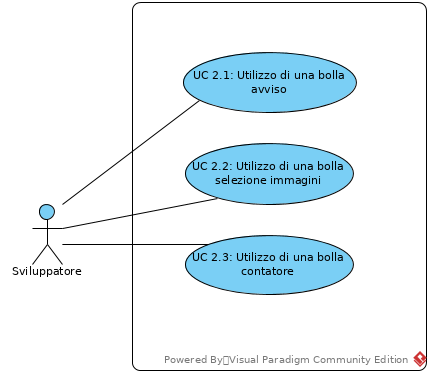
\includegraphics[scale=0.60]{Usecases/img/UC2.png}
	\caption{Caso d'uso UC 2: Utilizzo di bolle predefinite dell'SDK.}
\end{figure}

\FloatBarrier
\begin{itemize}
\item \textbf{Attori:} Sviluppatore.
\item \textbf{Descrizione:} Lo sviluppatore vuole utilizzare una bolla predefinita presente nell'SDK ovvero una tra le seguenti:
\begin{itemize}
\item Bolla avviso.
\item Bolla testo markdown.
\item Bolla lista.
\end{itemize} 
\item \textbf{Precondizione:} Lo sviluppatore vuole utilizzare una bolla predefinita presente nell'SDK. 
\item \textbf{Postcondizione:} Lo sviluppatore ha utilizzato una delle bolle predefinite presenti nella libreria di \progetto.
\item \textbf{Scenario principale:}
	\begin{itemize}
	\item{Utilizzo di una bolla avviso (UC 2.1).}
	\item{Utilizzo di una bolla testo markdown (UC 2.2).}
	\item{Utilizzo di una bolla lista (UC 2.3).}
	\end{itemize}
\end{itemize}
\subsubsection{Caso d'uso UC 2.1: Aggiunta di un metodo ad una bolla}

\FloatBarrier
\begin{itemize}
\item\textbf{Attori}: Sviluppatore.
\item\textbf{Descrizione}: Lo sviluppatore vuole aggiungere un nuovo metodo ad una bolla predefinita.
\item\textbf{Precondizione}: Lo sviluppatore vuole modificare il comportamento di una bolla predefinita presente in \progetto.
\item\textbf{Postcondizione}: Lo sviluppatore ha generato codice eseguibile per creare una nuova bolla derivata aggiungendo un metodo ad una bolla predefinita.
\end{itemize}
\subsubsection{Caso d'uso UC 2.2: Utilizzo di una bolla testo markdown}

\FloatBarrier
\begin{itemize}
\item\textbf{Attori}: Sviluppatore.
\item\textbf{Descrizione}: Lo sviluppatore vuole utilizzare una bolla predefinita di testo markdown. Questa bolla viene creata tramite l'inserimento di testo, scritto tramite la procedura di markdown.
\item\textbf{Precondizione}: Lo sviluppatore vuole utilizzare una bolla predefinita presente in \progetto.
\item\textbf{Postcondizione}: Lo sviluppatore ha generato codice eseguibile per creare una nuova bolla testo markdown.
\item\textbf{Scenario Principale}: Lo sviluppatore crea una bolla predefinita presente in \progetto.
\end{itemize}
\subsubsection{Caso d'uso UC 2.3: Utilizzo di una bolla lista}

\FloatBarrier
\begin{itemize}
\item\textbf{Attori}: Sviluppatore.
\item\textbf{Descrizione}: Lo sviluppatore vuole utilizzare la bolla lista predefinita. Questa bolla viene rappresenta la lista di elementi selezionabili.
\item\textbf{Precondizione}: Lo sviluppatore vuole utilizzare una bolla predefinita presente in \progetto.
\item\textbf{Postcondizione}: Lo sviluppatore ha generato codice eseguibile per creare una nuova bolla lista.
\item\textbf{Scenario Principale}: Lo sviluppatore crea una bolla predefinita presente in \progetto.
\end{itemize}
\subsection{Caso d'uso UC 3: Creazione di un widget personalizzato.}
\label{Caso d'uso UC 3: Creazione di un widget personalizzato.}

\FloatBarrier
\begin{itemize}
\item \textbf{Attori:} Sviluppatore.
\item \textbf{Descrizione:} Lo sviluppatore vuole creare un nuovo widget personalizzato.
\item \textbf{Precondizione:} Lo sviluppatore vuole creare un nuovo widget personalizzato. 
\item \textbf{Postcondizione:} Lo sviluppatore ha creato un nuovo widget personalizzato.
\item \textbf{Scenario principale:}
	\begin{itemize}
	\item{Lo sviluppatore vuole creare un nuovo widget personalizzato.}
	\end{itemize}
\end{itemize}

\newpage
\subsection{Caso d'uso UC 4: Applicazione demo lista-spesa.}
\label{Caso d'uso UC 4: Applicazione demo lista-spesa.}
\begin{figure}[ht]
	\centering
	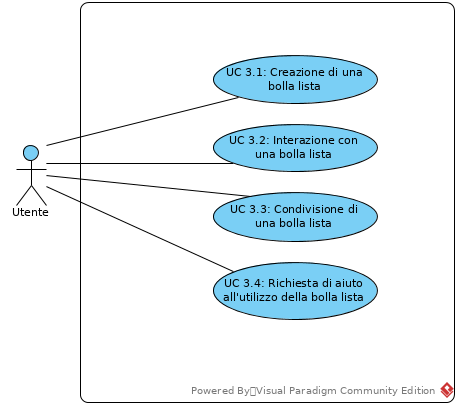
\includegraphics[scale=0.60]{Usecases/img/UC4.png}
	\caption{Caso d'uso UC 4: Applicazione demo lista spesa.}
\end{figure}



\FloatBarrier
\begin{itemize}
\item \textbf{Attori:} Utente.
\item \textbf{Descrizione:} L'utente utilizza l'applicazione demo lista-spesa.
\item \textbf{Precondizione:} L'utente vuole utilizzare l'applicazione demo lista-spesa. 
\item \textbf{Postcondizione:} L'utente ha utilizzato l'applicazione demo lista-spesa.
\item \textbf{Scenario principale:}
	\begin{itemize}
	\item{Creazione di una bolla lista-spesa (UC 4.1).}
	\item{Interazione con una bolla lista-spesa (UC 4.2).}
	\item{Condivisione di una bolla lista-spesa (UC 4.3).}
	\item{Richiesta di aiuto all'utilizzo della bolla lista spesa (UC 4.4).}
	\end{itemize}


\end{itemize}
\subsubsection{Caso d'uso UC 4.1: Configurazione di una bolla lista-spesa}
\label{Caso d'uso UC 4.1: Configurazione di una bolla lista-spesa}
\begin{figure}[ht]
	\centering
	\includegraphics[scale=0.80]{Usecases/img/{UC4.1}.png}
	\caption{Caso d'uso UC 4.1: Configurazione di una bolla lista-spesa}
\end{figure}
\FloatBarrier
\begin{itemize}
\item\textbf{Attori}: Creatore della lista.
\item\textbf{Descrizione}: L'attore crea la bolla lista-spesa e la configura.
\item\textbf{Precondizione}: L'attore vuole creare una bolla lista-spesa.
\item\textbf{Postcondizione}: Lo sviluppatore ha creato una bolla lista-spesa configurata.
\item\textbf{Estensioni}:
\begin{itemize}
		\item Impostazione del nome della lista a default(UC 4.1.2).
	\end{itemize}
	
\item\textbf{Scenario principale}:
	\begin{itemize}
		\item L'attore imposta il nome della lista-spesa(UC 4.1.1).
		\item L'attore imposta l'immagine della lista-spesa(UC 4.1.3).
	\end{itemize}
\item\textbf{Scenario alternativo}:
	\begin{itemize}
		\item L'attore non imposta il nome della lista oppure non lo imposta in modo non corretto(UC 4.1.2).
	\end{itemize}

\end{itemize}

\paragraph{Caso d'uso UC 4.1.1 Impostazione del nome della lista.}
	\begin{itemize}
	\item\textbf{Attori}: Creatore della lista.
		\item\textbf{Descrizione}: L'attore imposta il nome della lista.
		\item\textbf{Precondizione}: L'attore sta creando una bolla lista-spesa.
		\item\textbf{Postcondizione}: La bolla viene configurata con un nome desiderato.
		\item\textbf{Estensioni}: Impostazione del nome della lista a default(UC 4.1.2).
		\item\textbf{Scenario principale:} L'attore che sta creando la lista imposta il nome desiderato(UC 4.1.1).
		\item\textbf{Scenario alternativo:} L'attore che sta creando la lista non imposta il nome(UC 4.1.2)
		
	\end{itemize}

\paragraph{Caso d'uso UC 4.1.2 Impostazione del nome della lista a default.}
	\begin{itemize}
	\item\textbf{Attori}: Creatore della lista.
		\item\textbf{Descrizione}: La bolla viene impostata con un nome di default.
		\item\textbf{Precondizione}: L'attore non imposta il nome della lista oppure non lo imposta in modo non corretto.
		\item\textbf{Postcondizione}: La bolla viene configurata con un nome di default.
		\item\textbf{Scenario principale}: Il nome della lista, a causa di un mancato inserimento, viene impostato a default(UC 4.1.2).
		
	\end{itemize}
	
	
\paragraph{Caso d'uso UC 4.1.3 Impostazione dell'immagine della lista.}
	\begin{itemize}
	\item\textbf{Attori}: Creatore della lista.
		\item\textbf{Descrizione}: L'attore imposta l'immagine della lista.
		\item\textbf{Precondizione}: L'attore sta creando una bolla lista-spesa.
		\item\textbf{Postcondizione}: La bolla viene configurata con l'immagine desiderata.
		
		\item\textbf{Scenario principale:} L'attore che sta creando la lista imposta l'immagine desiderata(UC 4.1.3).
		
		
	\end{itemize}
	
\newpage
\subsubsection{Caso d'uso UC 4.2: Interazione con la bolla lista-spesa.}
\label{Caso d'uso UC 4.2: Interazione con la bolla lista-spesa.}
\begin{figure}[ht]
	\centering
	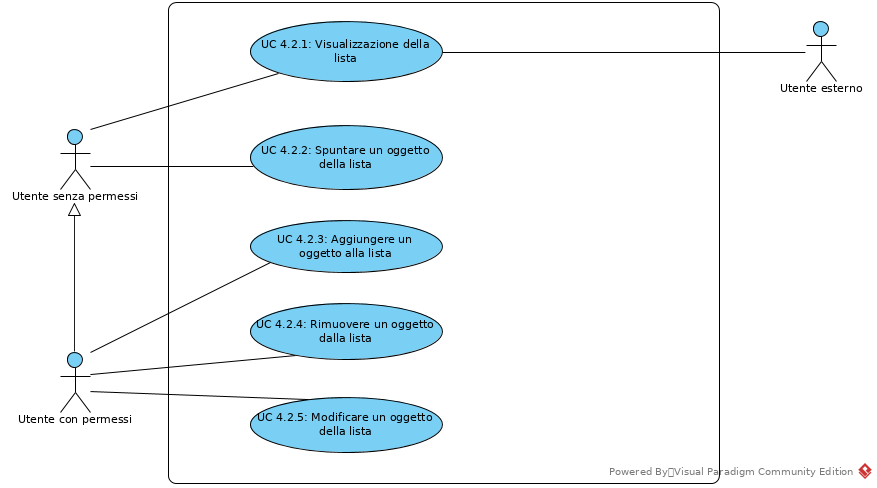
\includegraphics[scale=0.60]{Usecases/img/UC4.2.png}
	\caption{Caso d'uso UC 4.2: Interazione con la bolla lista-spesa.}
\end{figure}

\FloatBarrier
\begin{itemize}
\item \textbf{Attori:} Utente senza permessi, Utente con permessi, Utente esterno.
\item \textbf{Descrizione:} L'utente vuole interagire con la bolla lista-spesa e in base al tipo di utente potrà eseguire diverse azioni tra cui:
\begin{itemize}
\item Visualizzare la lista.
\item Spuntare un oggetto della lista.
\item Aggiungere un oggetto alla lista.
\item Rimuovere un oggetto dalla lista.
\item Modificare un oggetto della lista.
\end{itemize}
\item \textbf{Precondizione:} L'utente vuole interagire con la bolla lista-spesa. 
\item \textbf{Postcondizione:} L'utente ha interagito con la bolla lista-spesa con le modalità che la tipologia d'utente di cui fa parte permette.
\item \textbf{Scenario principale:}
	\begin{itemize}
	\item{Visualizzazione della lista (UC 4.2.1).}
	\item{Spunta di un oggetto della lista (UC 4.2.2).}
	\item{Aggiunta di un oggetto alla lista (UC 4.2.3).}
	\item{Rimozione di un oggetto dalla lista (UC 4.2.4).}
	\item{Richiesta di aiuto all'utilizzo della bolla lista spesa (UC 4.2.5).}
	\end{itemize}
\end{itemize}
\subsection{Caso d'uso UC 4.2.3: Aggiunta di un oggetto alla lista.}
\label{Caso d'uso UC 4.2.3: Aggiunta di un oggetto alla lista.}

\FloatBarrier
\begin{itemize}
\item \textbf{Attori:} Utente con permessi.
\item \textbf{Descrizione:} L'utente vuole aggiungere un oggetto alla bolla lista-spesa.
\item \textbf{Precondizione:} L'utente vuole aggiungere un oggetto alla bolla lista-spesa. 
\item \textbf{Postcondizione:} L'utente ha aggiunto un oggetto alla bolla lista-spesa.
\item \textbf{Scenario principale:}
	\begin{itemize}
	\item{L'utente aggiunge un oggetto alla bolla lista-spesa.}
	\end{itemize}
\end{itemize}
\paragraph{Caso d'uso UC 4.2.5: Modificare un oggetto della lista}
\label {Caso d'uso UC 4.2.5: Modificare un oggetto della lista}
\begin{figure}[ht]
	\centering
	\includegraphics[scale=0.80]{Usecases/img/{UC4.2.5}.png}
	\caption {Caso d'uso UC 4.2.5: Modificare un oggetto della lista}
\end{figure}
\FloatBarrier
\begin{itemize}
\item\textbf{Attori}: Utente con permessi.
\item\textbf{Descrizione}: L'attore modifica un oggetto della lista
\item\textbf{Precondizione}: L'attore ha i permessi per la modifica di un oggetto della lista.
\item\textbf{Postcondizione}: L'oggetto della lista viene modificato.
\item\textbf{Estensioni}:
	\begin{itemize}
		\item Visualizzazione messaggio d'errore(UC 4.2.5.2).
		\item Impostazione della quantità di prodotto richiesta a default(UC 4.2.5.7).
		\item Impostazione dell'unità di misura della quantità richiesta a default(UC 4.2.5.9). 
	\end{itemize}

	
\item\textbf{Scenario principale}:
	\begin{itemize}
		\item Modifica del nome del prodotto(UC 4.2.5.1).
		\item Modifica dell'immagine del prodotto(UC 4.2.5.3).
		\item Modifica della descrizione del prodotto(UC 4.2.5.4).
		\item Modifica delle note relative al prodotto(UC 4.2.5.5).
		\item Modifica della quantità richiesta di prodotto(UC 4.2.5.6).
		\item Modifica dell'unità di misura relativa alla quantità richiesta di prodotto(UC 4.2.5.8).
	\end{itemize}
\item\textbf{Scenario alternativo}:
	\begin{itemize}
		\item L'attore visualizza un messaggio d'errore a causa del mancato inserimento del nome del prodotto(UC 4.2.5.2).
		\item La quantità di prodotto viene aggiornata a default a causa del mancato inserimento di essa(UC 4.2.5.7).
		\item L'unità di misura della quantità di prodotto viene aggiornata a default a causa del mancato inserimento di essa(UC 4.2.5.9).
	\end{itemize}

\end{itemize}


\subparagraph{Caso d'uso UC 4.2.5.2 Visualizzazione messaggio d'errore.}
	\begin{itemize}
		\item\textbf{Attori}: Creatore della lista.
		\item\textbf{Descrizione}: L' attore visualizza un messaggio d'errore a causa del mancato inserimento del nome del prodotto.
		\item\textbf{Precondizione}: L' attore non imposta il nome del prodotto che vuole modificare.
		\item\textbf{Postcondizione}: L' attore visualizza un messaggio d'errore.
		\item\textbf{Scenario principale}:
			\begin{itemize}
				\item L'attore visualizza un messaggio d'errore. 
			\end{itemize}
		
	\end{itemize}
	
\subparagraph{Caso d'uso UC 4.2.5.7 Impostazione della quantità di prodotto richiesta a default.}
	\begin{itemize}
		\item\textbf{Attori}: Creatore della lista.
		\item\textbf{Descrizione}: La quantità di prodotto richiesta viene impostata a default a causa del mancato inserimento di essa.
		\item\textbf{Precondizione}: L'attore non imposta la quantità di prodotto che vuole modificare.
		\item\textbf{Postcondizione}:Il prodotto modificato ha una quantità  impostata a default.
		\item\textbf{Scenario principale}:
			\begin{itemize}
				\item La quantità del prodotto viene impostata a default.
			\end{itemize}
		
	\end{itemize}
\subparagraph{Caso d'uso UC 4.2.5.9 Impostazione dell'unità di misura della quantità richiesta a default.}
	\begin{itemize}
		\item\textbf{Attori}: Creatore della lista.
		\item\textbf{Descrizione}: L'unità di misura della quantità di prodotto richiesta viene impostata a default a causa del mancato inserimento di essa.
		\item\textbf{Precondizione}: L'attore non imposta l'unità di misura della quantità di prodotto che vuole modificare.
		\item\textbf{Postcondizione}: Il prodotto ha un unità di misura impostata a default.
		\item\textbf{Scenario principale}:
			\begin{itemize}
				\item L'unità di misura della quantità del prodotto viene impostata a default.
			\end{itemize}
		
\end{itemize}

\subsection{Caso d'uso UC 4.3: Condivisione di una bolla lista-spesa.}
\label{Caso d'uso UC 4.3: Condivisione di una bolla lista-spesa.}
\begin{figure}[ht]
	\centering
	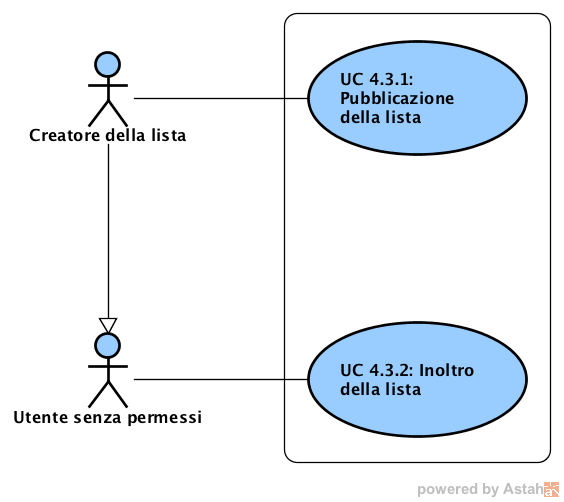
\includegraphics[scale=0.60]{Usecases/img/UC4.3.png}
	\caption{Caso d'uso UC 4.3: Condivisione di una bolla lista-spesa.}
\end{figure}

\FloatBarrier
\begin{itemize}
\item \textbf{Attori:} Utente.
\item \textbf{Descrizione:} L'utente utilizza l'applicazione demo lista-spesa.
\item \textbf{Precondizione:} L'utente vuole utilizzare l'applicazione demo lista-spesa. 
\item \textbf{Postcondizione:} L'utente ha utilizzato l'applicazione demo lista-spesa.
\item \textbf{Scenario principale:}
	\begin{itemize}
	\item{Creazione di una bolla lista-spesa (UC 4.1).}
	\item{Interazione con una bolla lista-spesa (UC 4.2).}
	\item{Condivisione di una bolla lista-spesa (UC 4.3).}
	\item{Richiesta di aiuto all'utilizzo della bolla lista spesa (UC 4.4).}
	\end{itemize}
\end{itemize}
\paragraph{Caso d'uso UC 4.3.1: Pubblicazione della lista.}
\label{Caso d'uso UC 4.3.1: Pubblicazione della lista.}

\FloatBarrier
\begin{itemize}
\item \textbf{Attori:} Creatore della lista.
\item \textbf{Descrizione:} Il Creatore della lista vuole pubblicare la bolla lista-spesa creata e può farlo in due modi:
\begin{itemize}
\item Pubblicando la bolla lista-spesa a un gruppo.
\item Pubblicando la bolla lista-spesa ad un utente.
\end{itemize}
\item \textbf{Precondizione:} Il Creatore della lista vuole pubblicare la bolla lista-spesa creata. 
\item \textbf{Postcondizione:} Il Creatore della lista ha pubblicato la bolla lista-spesa creata.
\item \textbf{Scenario principale:}
	\begin{itemize}
	\item{Pubblicazione della lista a un gruppo (UC 4.3.1.1).}
	\item{Pubblicazione della lista ad un utente (UC 4.3.1.4).}
	\end{itemize}
\end{itemize}
\subsection{Caso d'uso UC 4.3.1.1: Pubblicazione della lista a un gruppo.}
\label{Caso d'uso UC 4.3.1.1: Pubblicazione della lista a un gruppo.}

\FloatBarrier
\begin{itemize}
\item \textbf{Attori:} Creatore della lista.
\item \textbf{Descrizione:} Il Creatore della lista vuole pubblicare la bolla lista-spesa creata a un gruppo.
\item \textbf{Precondizione:} Il Creatore della lista vuole pubblicare la bolla lista-spesa creata a un gruppo. 
\item \textbf{Postcondizione:} Il Creatore della lista ha pubblicato a un gruppo la bolla lista-spesa creata.
\item \textbf{Inclusioni:}
	\begin{itemize}
	\item{Concessione ai partecipanti del gruppo dei permessi (UC 4.3.1.2).}
	\end{itemize}
\item \textbf{Scenario principale:}
	\begin{itemize}
	\item{Concessione ai partecipanti del gruppo dei permessi (UC 4.3.1.2).}
	\end{itemize}
\end{itemize}
\subparagraph{Caso d'uso UC 4.3.1.2: Concessione ai partecipanti del gruppo dei permessi.}
\label{Caso d'uso UC 4.3.1.2: Concessione ai partecipanti del gruppo dei permessi.}

\FloatBarrier
\begin{itemize}
\item \textbf{Attori:} Creatore della lista.
\item \textbf{Descrizione:} Il Creatore della lista vuole concedere ad alcuni partecipanti del gruppo i permessi di interazione con la bolla lista-spesa creata.
\item \textbf{Precondizione:} Il Creatore della lista vuole concedere ad alcuni partecipanti del gruppo i permessi di interazione con la bolla lista-spesa creata. 
\item \textbf{Postcondizione:} Il Creatore della lista ha concesso ad alcuni partecipanti del gruppo i permessi di interazione con la bolla lista-spesa creata.
\item \textbf{Estensioni:}
	\begin{itemize}
	\item{Permessi concessi a nessun partecipante (UC 4.3.1.3).}
	\end{itemize}
\item \textbf{Scenario principale:}
\begin{itemize}
\item Il Creatore della lista concede ad alcuni partecipanti del gruppo i permessi di interazione con la bolla lista-spesa creata.
\end{itemize}
\item \textbf{Scenario alternativo:}
	\begin{itemize}
	\item{Permessi concessi a nessun partecipante (UC 4.3.1.3).}
	\end{itemize}
\end{itemize}
\subsection{Caso d'uso UC 4.3.1.3: Permessi concessi a nessun partecipante.}
\label{Caso d'uso UC 4.3.1.3: Permessi concessi a nessun partecipante.}

\FloatBarrier
\begin{itemize}
\item \textbf{Attori:} Creatore della lista.
\item \textbf{Descrizione:} Il Creatore della lista non ha impostato per i partecipanti del gruppo i permessi di interazione con la bolla lista-spesa creata non concedendo di conseguenza i permessi di interazione con la bolla lista-spesa a nessun partecipante del gruppo.
\item \textbf{Precondizione:} Il Creatore della lista non ha impostato i permessi di interazione con la bolla lista-spesa creata per i partecipanti del gruppo.
\item \textbf{Postcondizione:} Il Creatore della lista non ha concesso a nessun partecipante del gruppo i permessi di interazione con la bolla lista-spesa.
\item \textbf{Scenario principale:}
\begin{itemize}
\item Il Creatore della lista non ha impostato per i partecipanti del gruppo i permessi di interazione con la bolla lista-spesa creata non concedendo di conseguenza i permessi di interazione con la bolla lista-spesa a nessun partecipante del gruppo.
\end{itemize}
\end{itemize}
\subsection{Caso d'uso UC 4.3.1.4: Pubblicazione della lista ad un utente.}
\label{Caso d'uso UC 4.3.1.4: Pubblicazione della lista ad un utente.}

\FloatBarrier
\begin{itemize}
\item \textbf{Attori:} Creatore della lista.
\item \textbf{Descrizione:} Il Creatore della lista vuole pubblicare la bolla lista-spesa creata ad un utente.
\item \textbf{Precondizione:} Il Creatore della lista vuole pubblicare la bolla lista-spesa creata ad un utente. 
\item \textbf{Postcondizione:} Il Creatore della lista ha pubblicato ad un utente la bolla lista-spesa creata.
\item \textbf{Inclusioni:}
	\begin{itemize}
	\item{Concessione all'utente dei permessi (UC 4.3.1.5).}
	\end{itemize}
	\item \textbf{Scenario principale:}
	\begin{itemize}
	\item{Concessione all'utente dei permessi (UC 4.3.1.5).}
	\end{itemize}
\end{itemize}
\subparagraph{Caso d'uso UC 4.3.1.5: Concessione all'utente dei permessi.}
\label{Caso d'uso UC 4.3.1.5: Concessione all'utente dei permessi.}

\FloatBarrier
\begin{itemize}
\item \textbf{Attori:} Creatore della lista.
\item \textbf{Descrizione:} Il Creatore della lista vuole concedere all'utente i permessi di interazione con la bolla lista-spesa creata.
\item \textbf{Precondizione:} Il Creatore della lista vuole concedere all'utente i permessi di interazione con la bolla lista-spesa creata. 
\item \textbf{Postcondizione:} Il Creatore della lista ha concesso all'utente i permessi di interazione con la bolla lista-spesa creata.
\item \textbf{Estensioni:}
	\begin{itemize}
	\item{Permessi non concessi all'utente (UC 4.3.1.6).}
	\end{itemize}
\item \textbf{Scenario principale:}
\begin{itemize}
\item Il Creatore della lista concede all'utente i permessi di interazione con la bolla lista-spesa creata.
\end{itemize}
\item \textbf{Scenario alternativo:}
\begin{itemize}
\item Permessi non concessi all'utente (UC 4.3.1.6).
\end{itemize}
\end{itemize}
\subparagraph{Caso d'uso UC 4.3.1.6: Permessi non concessi all'utente.}
\label{Caso d'uso UC 4.3.1.6: Permessi non concessi all'utente.}

\FloatBarrier
\begin{itemize}
\item \textbf{Attori:} Creatore della lista.
\item \textbf{Descrizione:} Il Creatore della lista non ha impostato per l'utente i permessi di interazione con la bolla lista-spesa creata non concedendo di conseguenza i permessi di interazione con la bolla lista-spesa all'utente.
\item \textbf{Precondizione:} Il Creatore della lista non ha impostato i permessi di interazione con la bolla lista-spesa creata per l'utente.
\item \textbf{Postcondizione:} Il Creatore della lista non ha concesso all'utente i permessi di interazione con la bolla lista-spesa.
\item \textbf{Scenario principale:}
\begin{itemize}
\item Il Creatore della lista non ha impostato per l'utente i permessi di interazione con la bolla lista-spesa non concedendo di conseguenza i permessi di interazione con la bolla lista-spesa all'utente.
\end{itemize}
\end{itemize}